\documentclass[12pt]{article}
\usepackage[T1]{fontenc}
\usepackage[margin=2cm]{geometry}

\usepackage{amssymb}
\usepackage{amsmath}
\usepackage{tcolorbox}
\usepackage{xcolor}
\usepackage{framed}
\usepackage{euscript}
\usepackage{float}

\usepackage{verbatim}
\usepackage{mathrsfs}
\usepackage{graphicx}
\usepackage{multicol}

\usepackage{bbm,txfonts}
\usepackage{float}


\usepackage{titletoc}
\usepackage{tikz}
\usepackage{xspace}

\usepackage{enumitem}

\newcommand{\answer}{\vspace*{4pt} \noindent{\bf Solution: }}

\newcommand{\bb}[1]{\mathbb{#1}}
\renewcommand{\v}[1]{\boldsymbol{#1}}
\newcommand{\m}[1]{\mathbf{#1}}
\renewcommand{\c}[1]{\mathcal{#1}}
\usepackage{upquote}


\renewcommand{\tilde}{\widetilde}
\newcommand{\halmos}{\vspace{3mm} \hfill \mbox{$\Box$}}

\newcommand{\Var}{\mathbb{V}\mathrm{ar}}
\newcommand{\var}{\Var}

\newcommand{\Cov}{\mathbb{C}\mathrm{ov}}
\newcommand{\cov}{\Cov}

\renewcommand{\epsilon}{\varepsilon}
\renewcommand{\rho}{\varrho}
\renewcommand{\log}{\ln}
\renewcommand{\hat}{\widehat}

\newcommand{\iid}{\text{iid }}


% Bernoulli distribution
\newcommand{\Ber}{{\sf Ber}}
\newcommand{\ber}{\Ber}

% Binomial distribution
\newcommand{\Bin}{{\sf Bin}}
\newcommand{\bin}{\Bin}

% Cauchy distribution
\newcommand{\Cauchy}{{\sf Cauchy}}

% Negative binomial distribution
\newcommand{\NegBin}{{\sf NegBin}}

% Multinomial distribution
\newcommand{\Mnom}{{\sf Mnom}}
\newcommand{\mnom}{\Mnom}

% Geometric distribution
\newcommand{\Geo}{{\sf Geom}}
\newcommand{\geo}{\Geo}
\newcommand{\Geom}{\Geo}
\newcommand{\geom}{\Geo}
\newcommand{\G}{\Geo}

% Hypergeometric distribution
\newcommand{\Hyp}{{\sf Hyp}}

% Poisson distribution
\newcommand{\Poi}{{\sf Poi}}
\newcommand{\poi}{\Poi}
\newcommand{\Po}{\Poi}
\newcommand{\po}{\Poi}

% Uniform distribution (continuous)
\newcommand{\U}{\EuScript{U}}

% Exponential distribution
\newcommand{\Ex}{{\sf Exp}}
\newcommand{\ex}{\Ex}

% Normal / Gaussian distribution
\newcommand{\Nor}{\EuScript{N}}
\newcommand{\nor}{\Nor}

% Pareto distribution
\newcommand{\Pareto}{{\sf Pareto}}
\newcommand{\pareto}{\Pareto}

% Negative hypergeometric distribution
\newcommand{\NegHyp}{{\sf NegHyp}}

% Student's t distribution
\newcommand{\Student}{{\sf t}}
\newcommand{\student}{\Student}

% Gamma distribution
\newcommand{\Gam}{{\sf Gamma}}
\newcommand{\gam}{\Gam}

% Discrete uniform distribution
\newcommand{\DU}{{\sf DU}}

% Generic distribution
\newcommand{\Dist}{{\sf Dist}}

\newcommand{\Em}{{\mathbb E}}  % expectation
\newcommand{\Pm}{{\mathbb P}}  % probability measure
\newcommand{\R}{{\mathbb R}}

\newcommand{\gvn}{\,|\,}  % conditional (given)

\newcommand{\e}{\mathrm{e}} %Euler's e

\newcommand{\ds}{\displaystyle}

\newcommand{\di}{\mathrm{d}}  % use for differential symbol


\newcommand{\approxsim}{\stackrel{\mathrm{approx.}}{\sim}}

\newcommand{\iidsim}{\stackrel{\mathrm{iid}}{\sim}}
\newcommand{\simiid}{\iidsim}
\newcommand{\simiidt}{{\:{\sim}_{\mathrm{iid}}\:}}

%% Correlation
\newcommand{\Corr}{\mathrm{Corr}}
\newcommand{\corr}{\Corr}


\usepackage{cprotect}
\RequirePackage[formats]{listings}\RequirePackage{textcomp}

\lstnewenvironment{Pout}{%
  \lstset{backgroundcolor=\color{outcol},
  aboveskip= -2pt,  
  xleftmargin = 4pt,
  xrightmargin = 4pt,
  frame=single,
  upquote,
  framerule=1pt,
  basicstyle=\footnotesize\ttfamily,
  columns=fixed}}{}

%DK: See http://latexcolor.com/
\definecolor{applegreen}{rgb}{0.55, 0.41, 0.0}
\definecolor{gray1}{rgb}{0.98, 0.98, 0.98}
\definecolor{black}{rgb}{0, 0, 0}
\definecolor{cream}{rgb}{1.0, 0.99, 0.82}
\definecolor{islamicgreen}{rgb}{0.0, 0.56, 0.0}
\definecolor{vlgray}{gray}{0.9}
\definecolor{lgray}{gray}{0.7}
\definecolor{outcol}{gray}{0.9}

\tcbuselibrary{listings,skins,breakable,theorems}

\newenvironment{PC}{%
\tcblisting{breakable,listing only,colback=cream, enhanced, sharpish
corners,  boxrule=1pt,after, listing options =
   {language=Python,
  basicstyle=\footnotesize\ttfamily,        % the size of the fonts that are used for the code
  numbers=none,                   % where to put the line-numbers
%  numberstyle=\tiny\color{blue},  % the style that is used for the line-numbers
  xleftmargin=-10pt,
  aboveskip=-4pt,
  belowskip=-6pt,
  columns=fixed,
  basewidth=5pt,                     %separation of letters
%  stepnumber=1,                % the step between two line-numbers. If it's 1, each line will be numbered
%  numbersep=7pt,                  % how far the line-numbers are from the code
  backgroundcolor=\color{cream},  % choose the background color. You must add \usepackage{color}
  showspaces=false,               % show spaces adding particular underscores
  showstringspaces=false,         % underline spaces within strings
  showtabs=false,                 % show tabs within strings adding particular underscores
  %frame=single,                   % adds a frame around the code
  %frame=shadowbox,
  %rulecolor=\color{black},        % if not set, the frame-color may be changed on line-breaks within not-black text (e.g. comments (green here))
  tabsize=2,                     % sets default tabsize to 2 spaces
 % captionpos=b,                  % sets the caption-position to bottom
  breaklines=true,                % sets automatic line breaking
  breakatwhitespace=false,        % sets if automatic breaks should only happen at whitespace
  %title=\lstname,                 % show the filename of files included with \lstinputlisting;
                                  % also try caption instead of title
  keywordstyle=\color{blue},      % keyword style
  upquote,     % very important to get right quote for cut/paste
  commentstyle=\color{islamicgreen},   % comment style
  stringstyle=\color{red},      % string literal style
 % escapeinside={\%*}{*)},         % if you want to add a comment within your code
  morekeywords={*,...}
  			 }
    		}
    	}
{\endtcblisting}







\usepackage{fvextra}
\DefineVerbatimEnvironment{Code}{Verbatim}{
    fontsize=\footnotesize, % Adjust font size
    breaklines=true,        % Enable line wrapping
    breakanywhere=true      % Allow breaking anywhere
}

\usepackage{fvextra}
\usepackage{booktabs} % <-- Add this line
\DefineVerbatimEnvironment{Code}{Verbatim}{
    fontsize=\footnotesize, % Adjust font size
    breaklines=true,        % Enable line wrapping
    breakanywhere=true      % Allow breaking anywhere
}


\begin{document}
\begin{center}

{\Large  {\bf MACHINE LEARNING (COMP7703)}

Assignment - Semester 1, 2025.

\vspace{20pt}

{\large \textbf{Student Name:} Volter Entoma}
\vspace{10pt}

{\large \textbf{Student ID:} 44782711}

}
\end{center}

\vspace{20pt}

\textbf{1. Introduction}
\\
There are many different machine learning algorithms, and many metrics to evaluate them. In this assignment, we will focus on the K-Nearest Neighbour (K-NN) algorithm, Random Forest, and Deep Neural Networks, and the accuracy of each model. We will also looks at the different metrics to evaluate the performance of each model, and use these metrics to compare the suitability of each model for the given data.

\vspace{20pt}

\textbf{2. Aims}
\begin{itemize}
	\item To understand the K-Nearest Neighbour (K-NN) algorithm.
	\item To understand the accuracy of the K-NN classifier.
	\item To understand the effect of data imbalance on the accuracy of the K-NN classifier.
	\item To understand how to use cross-validation to improve the accuracy of the K-NN classifier.
\end{itemize}

\vspace{20pt}

\textbf{3. Data}
\\
The data used in this assignment is the \texttt{TTSWING} dataset, which is the provided dataset for this assignment. The dataset contains the 34 features, which are the 34 different measuremeents of table tennis swings. The dataset also contains the height of the player, which is the target variable. The dataset is a CSV file, and can be read into Python using the \texttt{pandas} library. The dataset is split into three categories: high, medium, and low.

\vspace{20pt}

\textbf{3.1 Data split}
\\
The data is split into three height categories: high, medium, and low. The data is split into 60\% training data, 20\% testing data, and 20\% validation data. The training data is used to train the each model, the testing data is used to test the accuracy of each model, and the validation data is used to compare the performance of the models. 

\vspace{20pt}

\textbf{3.2 Data imbalance}
\\
After splitting the data, there is an imbalance in the amount of training data assigned to each category in height. There are 17364 (29.73\%) data points in the high, 40800 (42.03\%) data points in the medium, and 27450 (28.23\%) in the low category. This is a significant imbalance; this imbalance is problematic because many machine learning algorithms tend to be biased toward the majority class. This can result in poor predictive performance for the minority classes, as the model may learn to ignore them in favor of achieving higher overall accuracy. In imbalanced datasets, accuracy becomes a misleading metric, since a model can achieve high accuracy by simply predicting the majority class most of the time, while failing to correctly classify minority class instances. This is especially concerning when the minority classes are of particular interest or importance.
\\
The data imbalanced is addressed by the use of Synthetic Minority Over-sampling Technique (SMOTE) to generate synthetic data points for the low category. The SMOTE algorithm generates synthetic data points by interpolating between existing data points in the low category. This is done by selecting a random data point from the low category, and then selecting a random data point from the k nearest neighbours of that data point. The synthetic data point is then generated by taking a weighted average of the two data points.
\\
After applying SMOTE, the training data is balanced, with 24552 data points in each category. All subsequent analysis is performed on the balanced training data. The testing and validation data is not balanced, and is used to test the accuracy of the models.
 
\vspace{20pt}

\textbf{3.3 Data standardization}
\\
The data is standardized using the StandardScaler from the \texttt{sklearn} library. The StandardScaler standardizes the data by removing the mean and scaling to unit variance. This is done to ensure that all features have the same scale, and to improve the performance of the models.

% Insert figure of data distribution here
\begin{figure}[H]
\centering
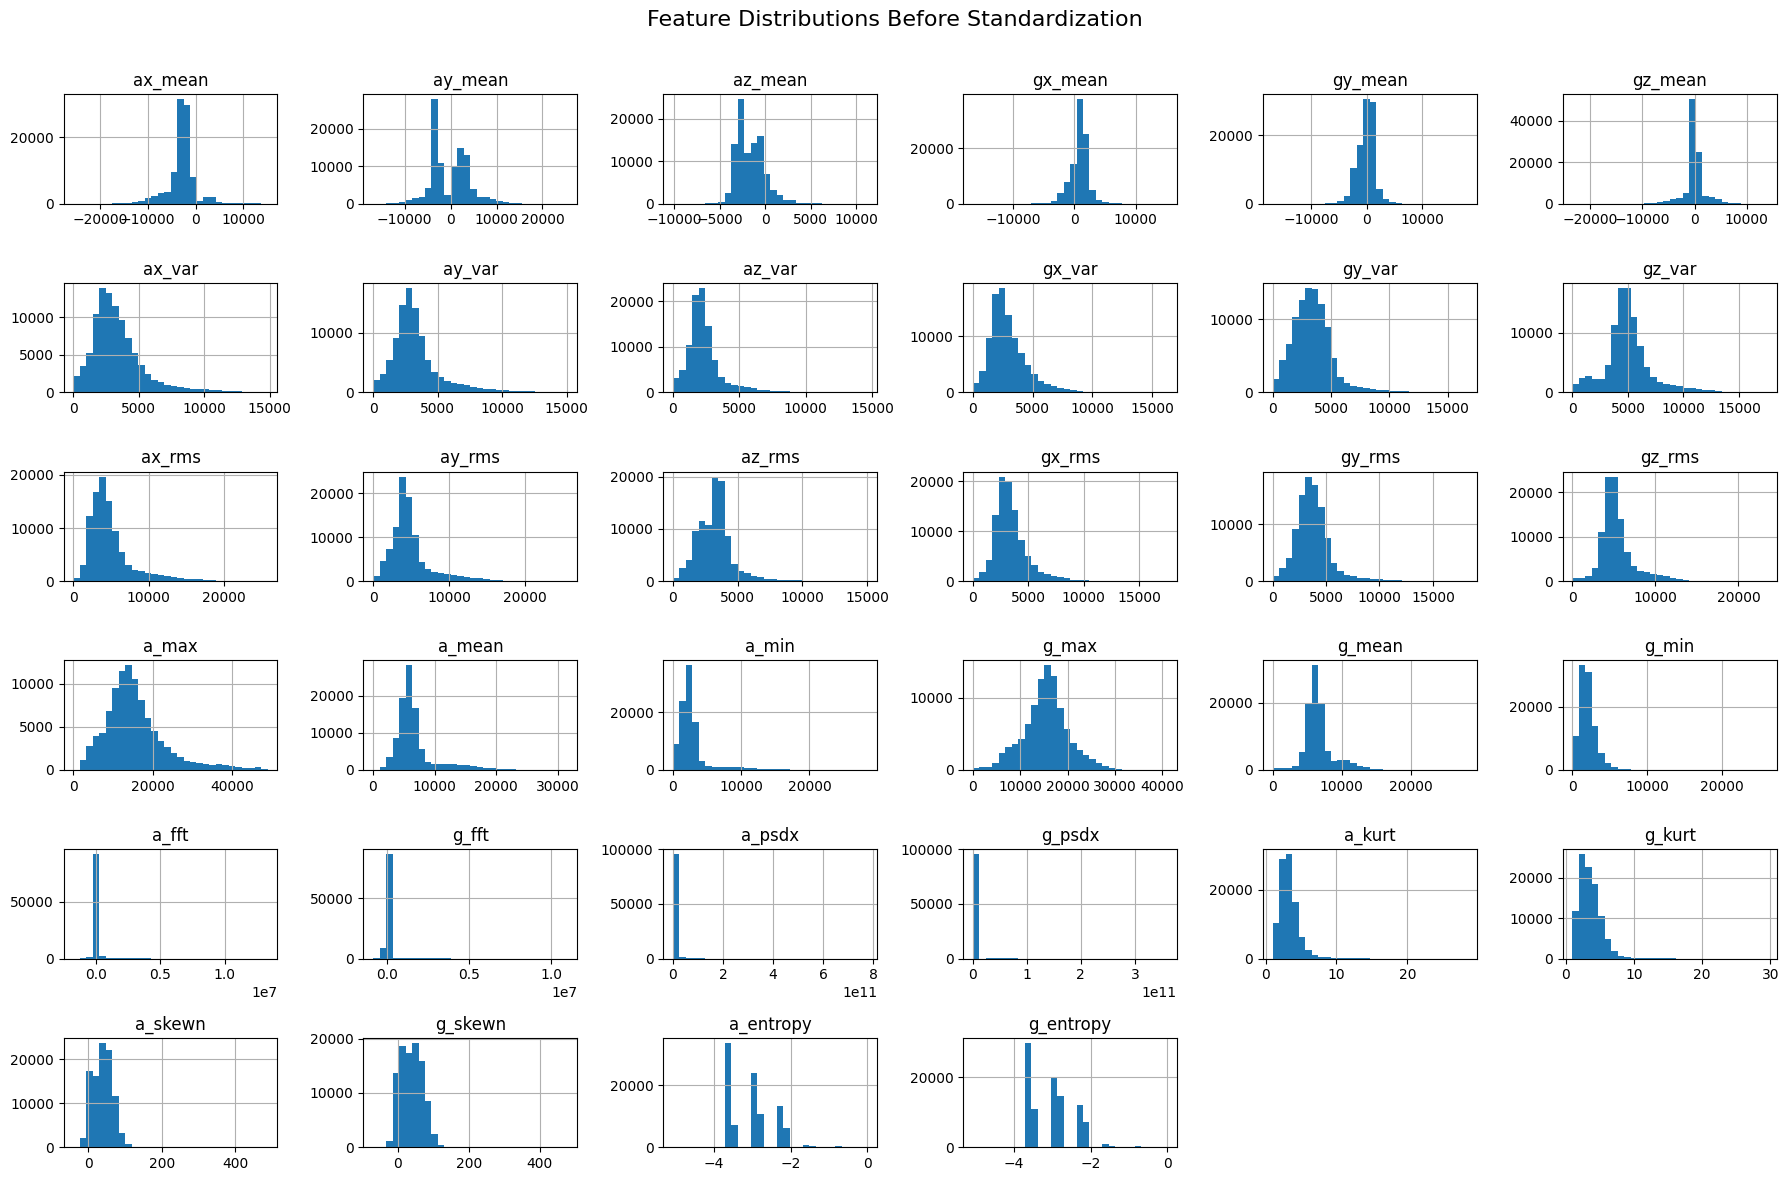
\includegraphics[width=1.0\textwidth]{figures/data_distribution.png}
\caption{Distribution of the data before standardization.}
\label{fig:data_distribution}
\end{figure}


\vspace{20pt}

\textbf{4. Principle Component Analysis}

To investigate the effect of dimensionality reduction on the accuracy of the models, we will use Principle Component Analysis (PCA) to reduce the dimensionality of the data. PCA is a linear transformation that transforms the data into a new coordinate system, where the first coordinate is the direction of maximum variance, the second coordinate is the direction of maximum variance orthogonal to the first coordinate, and so on. 

% Insert figure of Scree plot here
\begin{figure}[H]
\centering
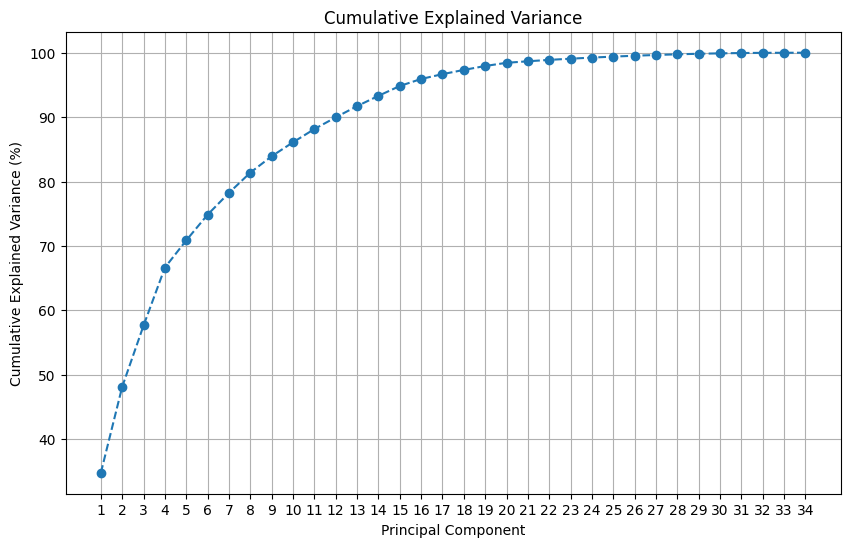
\includegraphics[width=0.8\textwidth]{figures/cum_var_scree.png}
\caption{Cumulative variance explained by each principal component.}
\label{fig:scree_plot}
\end{figure}

As shown in Figure \ref{fig:scree_plot}, approximately 95\% of the total variance is explained by the top 16 principal components. This allows us to reduce the dimensionality of our data from 34 dimensions to 16 dimensions while retaining the vast majority of the information content. 

\vspace{10pt}

By taking a look at the correlation matrix of the data, as shown in Figure \ref{fig:correlation_matrix}, we can see that there are many features that are highly correlated with each other. These off-diagonal correlations could explain why the PCA transformation is able to reduce the dimensionality of the data while retaining a high percentage of the variance.

% Insert figure of Correlation matrix here
\begin{figure}[H]
\centering
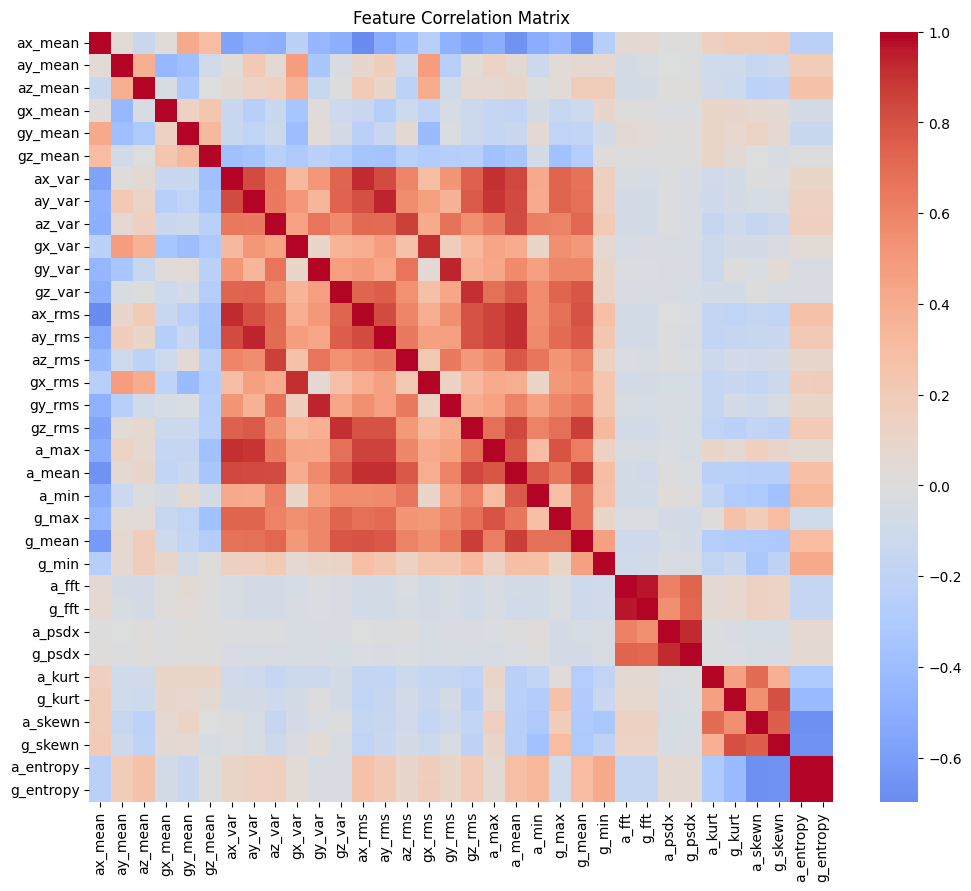
\includegraphics[width=0.8\textwidth]{figures/correlation_matrix.png}
\caption{Correlation matrix of the standardized data.}
\label{fig:correlation_matrix}
\end{figure}

Dimesnional eduction offers several benefits:

\begin{itemize}
    \item Reduced computational complexity in subsequent modeling
    \item Mitigation of the curse of dimensionality
    \item Removal of potentially noisy or redundant features
    \item Improved model interpretability
\end{itemize}

The effectiveness of this dimensionality reduction will be evaluated by comparing model performance on both the original and PCA-reduced datasets.

\vspace{20pt}

\textbf{5. K-NN classifier}

The K-Nearest Neighbour (K-NN) algorithm is a simple and effective machine learning algorithm that can be used for both classification and regression tasks. The K-NN algorithm works by finding the k nearest neighbours of a data point, and then predicting the class of the data point based on the classes of the k nearest neighbours. The K-NN algorithm is a non-parametric algorithm, which means that it does not make any assumptions about the distribution of the data. This makes the K-NN algorithm very flexible, and it can be used for a wide variety of tasks, including for our case of the classifying the height of a table tennis player based on their swing data.
\\
The K-NN algorithm was applied to the data to classify the height of the player based on their swing data.


\vspace{20pt}


\textbf{5.1 Accuracy of K-NN classifier}
\\
Using the data split outlined in Section 3.1, the K-NN classifier was trained on the training data, and then tested on the testing data. 

% Insert figure of K-NN accuracy here
\begin{figure}[H]
\centering
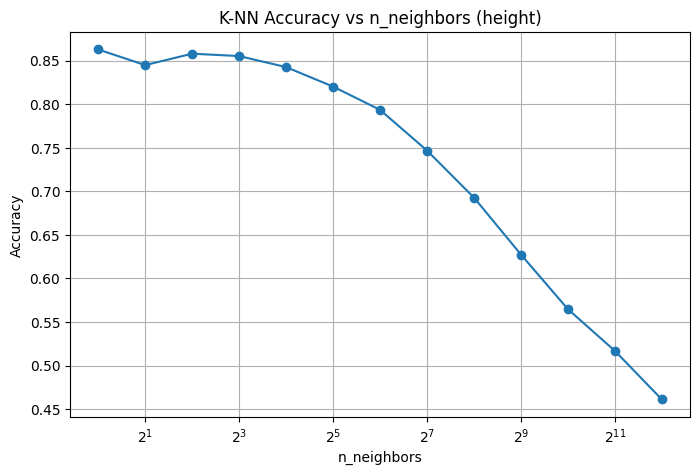
\includegraphics[width=0.8\textwidth]{figures/knn_accuracy.png}
\caption{Accuracy of K-NN classifier against the train and test data.}
\label{fig:knn_accuracy}
\end{figure}

The accuracy of the K-NN classifier is heavily dependent on the number of neighbours (k) used in the algorithm. Figure \ref{fig:knn_accuracy} shows the accuracy of the K-NN classifier reaches a maximum at 1 neighbour, and then decreases as the number of neighbours increases. This could be related to the high dimensionality of the data.
\\
The K-NN classifier is particularily sensitive to the curse of dimensionality; as the number of dimensions increases, point within the hyperspace are more likely to be equidistant from each other. This means that the K-NN algorithm is less able to distinguish between points, and hence the accuracy of the K-NN classifier decreases. This is a common problem with high dimensional data, and is one of the reasons why dimensionality reduction techniques such as PCA are used.
\\

We can confirm this by looking at the accuracy of the K-NN classifier on the PCA-reduced data. 

% Insert figure of K-NN accuracy on PCA-reduced data here
\begin{figure}[H]
\centering
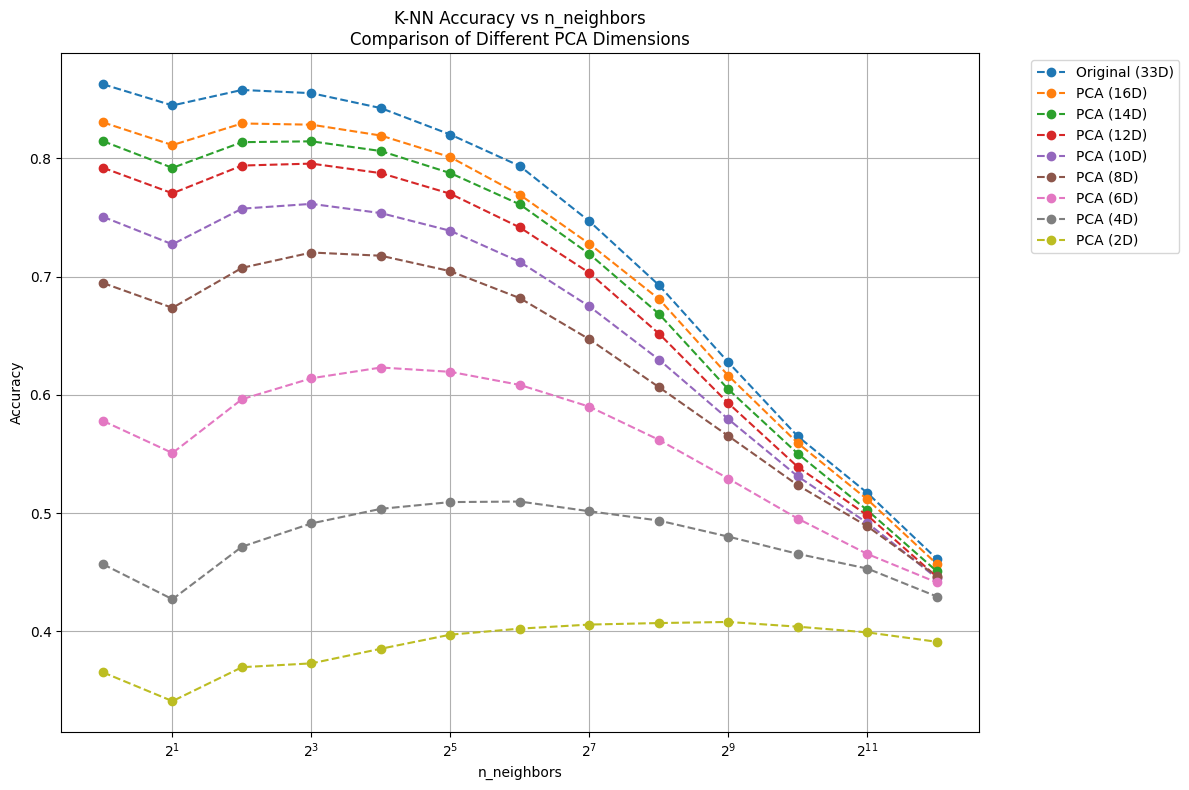
\includegraphics[width=0.9\textwidth]{figures/knn_accuracy_pca.png}
\caption{Accuracy of K-NN classifier on PCA-reduced data against the test data.}
\label{fig:knn_accuracy_pca}
\end{figure}


The accuracy of the K-NN classifier on the PCA-reduced data is shown in Figure \ref{fig:knn_accuracy_pca}. 
The curve for reduced data to 2-dimensions shows the best accuracy occurs with $2^9$ neighbour, which suggests that the points become more "spread-out" in 2-dimensions and the model is able to distinguish between different catgeories better as the number of neighbours increases. 
\\
However, despite the dimensionality reduction, the accuracy of the K-NN classifier is still highest at 1 neighbour, and then decreases as the number of neighbours increases. This suggests that the decrease in accuracy as neighbours increase is not solely due to the high dimensionality of the data, but also due to the nature of the K-NN algorithm on this particular dataset. This idea is supported by the fact that the curve for the PCA-reduced data (to 16 dimensions) is similar to the curve for the original data. 
\\
Additionally, the accuracy of the K-NN classifier decreases as the number of dimensions decreases. If the curse of dimensionality was a significant problem for this dataset, we would expect the accuracy to increase. This suggests that the curse of dimensionality is not a significant problem for this dataset, and that decreasing the number dimensions is not beneficial to the model, as it loses too much information.

\textbf{5.1.1 Computational time after dimensionality reduction}
\\
The computational time of the K-NN classifier is also significantly reduced after dimensionality reduction. The computational time of the K-NN classifier is largest

\vspace{20pt}

\textbf{5.2 K-Fold Cross-validation}
\\ 
The best accuracy of the K-NN classifier is achieved with one neighbour, and the accuracy is approximately 86.26\%. However, one neighbour could be overfitting the data, therefore is important to explore different sets of training and testing data, to see if the accuracy is consistent across different sets of data. This is done by using K-Fold Cross-validation, which splits the data into K different sets, and then trains and tests the model on each set. The accuracy of the model is then averaged over all K sets. 
\\
We use 10-fold cross-validation, which means that the data is split into 10 different sets, and then the model is trained and tested on each set. Note that the choice of the number of folds was arbitrary, and was chosen to be 10 because it is a common choice in the literature.
\\

% Insert figure of Accuracy of K-NN classifier with K-Fold Cross-validation here
\begin{figure}[H]
\centering
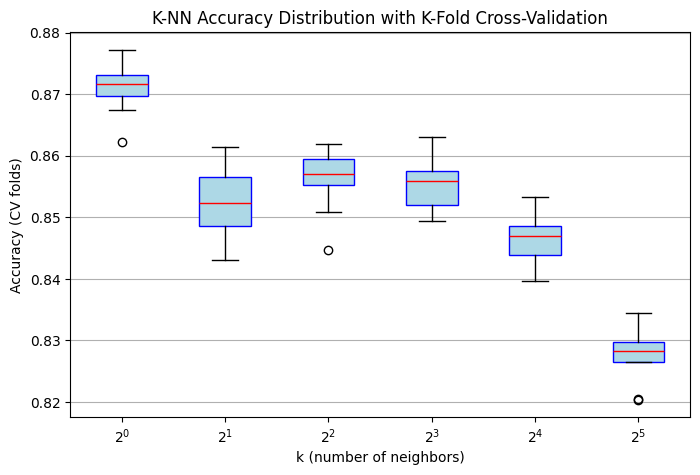
\includegraphics[width=0.8\textwidth]{figures/knn_accuracy_kfold.png}
\caption{Accuracy of K-NN classifier with K-Fold Cross-validation. Each box and whisker plots shows the spread of the accuracy against the test data across the 10 folds. The red line shows the mean accuracy across the 10 folds.}
\label{fig:knn_accuracy_kfold}
\end{figure}

The accuracy of the K-NN classifier with K-Fold cross-validation is shown in Figure \ref{fig:knn_accuracy_kfold}. With 10-fold cross-validation, the highest average accuracy occurs with one neighbour. Notably, the minimum accuracy across the 10 folds for one neighbour is approximately equal to the maximum accuracy observed for two, four, and eight neighbours. This suggests that one neighbour is indeed the optimal choice for this dataset.

Additionally, the variance in accuracy across folds for one neighbour is comparable to the variance observed for other values of k. If one neighbour were overfitting the data, we would expect to see significantly higher variance across the folds for k=1 compared to other values of k. Since this is not the case, we can conclude that, for this dataset, the K-NN classifier with one neighbour does not appear to overfit, as evidenced by the consistently low variance.
\\

\textbf{5.3 ROC curve}
\\
We use the k=1 K-NN model with the highest accuracy in the 10-fold cross-validation to plot the ROC curve. The ROC curve is a graphical representation of the performance of a binary classifier as the discrimination threshold is varied. It plots the true positive rate (TPR) against the false positive rate (FPR) at various threshold settings. The area under the ROC curve (AUC) is a single scalar value that summarizes the performance of the classifier across all thresholds.

% Insert figure of ROC curve here
\begin{figure}[H]
\centering
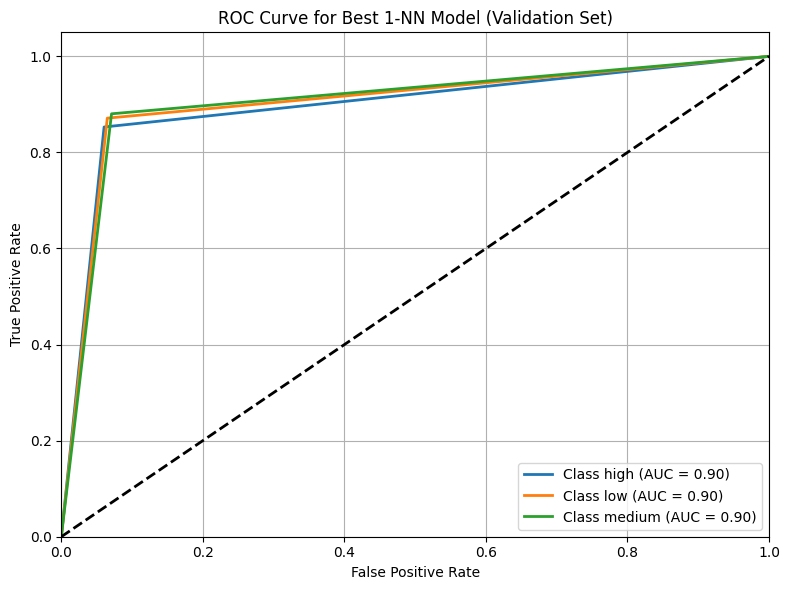
\includegraphics[width=0.8\textwidth]{figures/knn_roc_curve.png}
\caption{ROC curve for K-NN classifier with k=1.}
\label{fig:knn_roc_curve}
\end{figure}

The ROC curve for the K-NN classifier with k=1 is shown in Figure \ref{fig:knn_roc_curve}. The AUC for the K-NN classifier with k=1 is approximately 0.9 for all height categories. This indicates that the K-NN classifier with k=1 is a good classifier, as it has a high true positive rate and a low false positive rate. 
\\
The ROC curve itself is not very informative for one-neighbour K-NN, as it can only produce three points. The lack of points is due to the fact that the model outputs "hard" probabilityes (only 0 or 1) for each class, rather than "soft" probabilities, that would be possible for a higher number of neighbours. 
\\

\textbf{5.4 Confusion matrix}
\\
We can also use the same K-NN model to plot the confusion matrix using the validation data that was not used in the training or testing of the model. The confusion matrix is a table that is often used to describe the performance of a classification model on a set of data for which the true values are known. The confusion matrix shows the number of correct and incorrect predictions made by the model, broken down by class.

% Innsert figure of Confusion matrix here
\begin{figure}[h!]
\centering
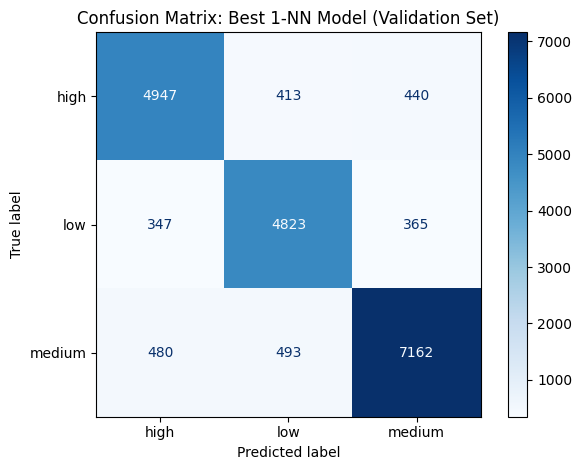
\includegraphics[width=1\textwidth]{figures/knn_confusion_matrix.png}
\caption{Confusion matrix for K-NN classifier with k=1. (Left) Confusion matrix against the raw validation set. (Right) Confusion matrix normalized by row.}
\label{fig:knn_confusion_matrix}
\end{figure}

The confusion matrix shows that the diagonal elements to be the largest, which indicates that the K-NN classifier with k=1 is able to correctly classify the majority of the data points.
\\
The off-diagonal elements are much smaller, which indicates that the K-NN classifier with k=1 is not making many incorrect predictions. This is a good sign, as it indicates that the K-NN classifier with k=1 is a good classifier for this dataset.
\\
The validation set has a significant imbalance in the number of data points in each category; similar to the raw training data, the medium category has the most data points, followed by the low and high categories. However, SMOTE was not applied to validation because artificially generating data points would give misleading performance metrics. Instead, the confusion matrix is normalized by row, which allows us to see the proportion of correct and incorrect predictions for each category. The normalized confusion matrix shows that the K-NN classifier with k=1 is able to correctly classify the majority of the data points in each category.
\\

\textbf{5.5 Precision, Recall, and F1 score}
\\
The precision, recall, and F1 score are three metrics that are commonly used to evaluate the performance of a classification model. The precision is the number of true positive predictions divided by the total number of positive predictions. The recall is the number of true positive predictions divided by the total number of actual positive instances. The F1 score is the harmonic mean of precision and recall.

\begin{table}[H]
\centering
\caption{Precision, Recall, and F1 Score for each class (Validation Set)}
\label{tab:knn_prf1}
\begin{tabular}{lcccc}
\toprule
Class      & Precision & Recall & F1-score \\
\midrule
high       & 0.86      & 0.85   & 0.85     \\
low        & 0.84      & 0.87   & 0.86     \\
medium     & 0.90      & 0.88   & 0.89     \\
\bottomrule
\end{tabular}
\end{table}

All three classes have a high precision, recall, and F1 score, which indicates that the K-NN classifier with k=1 is able to correctly classify the majority of the data points in each category. Additionally, the score are relatively balanced across all classes, which suggests that the K-NN classifier with k=1 is not biased towards any particular class, despite the imbalanced validation data.


\vspace{20pt}

\textbf{6. Random Forest Classifier}
\\
The Random Forest classifier is an ensemble learning method that constructs a multitude of decision trees during training and outputs the mode of the classes (classification) or mean prediction (regression) of the individual trees. It is particularly effective for high-dimensional datasets and can handle both categorical and continuous variables. The Random Forest algorithm is robust to overfitting, especially when the number of trees in the forest is large. In this section, we will explore the performance of the Random Forest classifier on the TTSWING dataset.
\\
Random Forest builds many decision trees using random subsets of the data and features, and aggregates their predictions. The quality of each split in a tree is measured using criteria such as Gini impurity (for classification), Entropy (information gain), or Mean Squared Error (for regression). 
\\
To keep this report within reasonable constraints, we will only explore the Gini impurity, and explore other parameters within the Random Forest classifier. The Gini impurity is a measure of how often a randomly chosen element from the set would be incorrectly labeled if it was randomly labeled according to the distribution of labels in the subset. 

\vspace{20pt}

\textbf{6.1 Accuracy of Random Forest Classifier}
\\
The Random Forest classifier was trained on the balanced and scaled training data, and then tested on the testing data. Various values of the number of trees in the forest (10, 50, 100, 200, 500, 800, and 1400), and the maximum depth of the trees (5, 10, 20, 30, 40, and no limit) were explored. The accuracy of the Random Forest classifier was then calculated for each combination of parameters.

% Insert figure of Random Forest accuracy here
\begin{figure}[H]
\centering
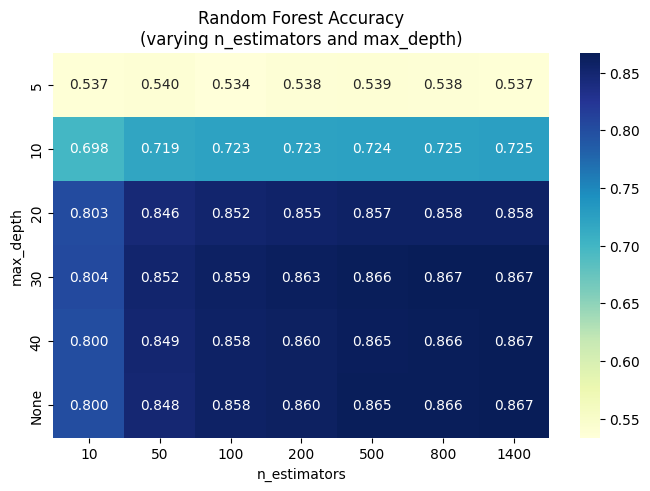
\includegraphics[width=1.0\textwidth]{figures/rf_accuracy.png}
\caption{Accuracy of Random Forest classifier against the train and test data.}
\label{fig:rf_accuracy}
\end{figure}

We can see from Figure \ref{fig:rf_accuracy} that the accuracy of the Random Forest classifier increases as the number of trees in the forest increases, and as the maximum depth of the trees increases. This is expected, as more trees and deeper trees allow for more complex decision boundaries to be learned. However, there is a point of diminishing returns, where increasing the number of trees or depth does not significantly improve accuracy.
\\
However, as a caveat, the accuracy of the Random Forest classifier is not garaunteed to increase as the maximum depth of the trees increases. This is because deeper trees are more likely to overfit the data, and hence the accuracy may decrease as the maximum depth increases. This is particularly evident in all trees that were explored - the accuracy of the Random Forest classifier peaks at a maximum depth of either 20 or 30, then decreases slightly as the maximum depth increases. This suggests that the Random Forest classifier is able to learn complex decision boundaries without overfitting the data, but that there is a limit to how complex the decision boundaries can be before overfitting occurs.

\vspace{20pt}

\textbf{6.1.1 Computational time after dimensionality reduction}
\\
A big drawback with increasing the number of trees and the maximum depth of the trees is the computational time. The computational time of the Random Forest classifier is significantly increased as the number of trees and maximum depth increases. This is because each tree in the forest must be trained on the data, and each tree must be traversed to make a prediction. This can be mitigated by using dimensionality reduction techniques such as PCA, which reduces the number of features in the data, and hence reduces the computational time.

% Insert figure of Random Forest accuracy on PCA-reduced data here
\begin{figure}[H]
\centering
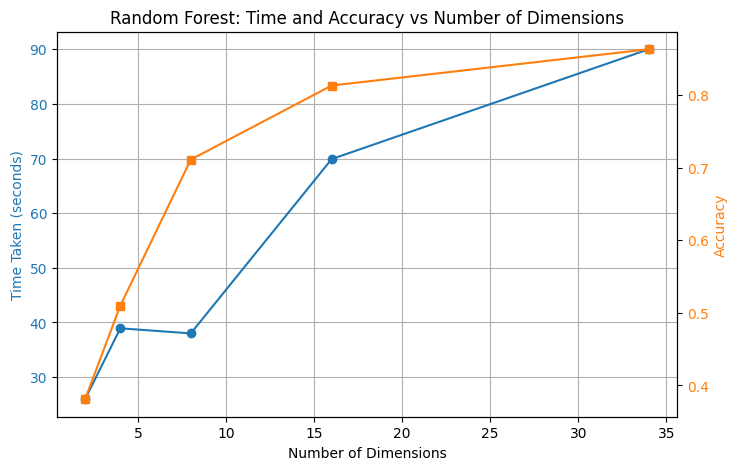
\includegraphics[width=0.9\textwidth]{figures/rf_accuracy_pca.png}
\caption{Accuracy of Random Forest classifier on PCA-reduced data. The model parameters were set to 200 trees and a maximum depth of 30.}
\label{fig:rf_accuracy_pca}
\end{figure}

When the data is reduced to 16-dimensions using PCA, the computational time of the Random Forest classifier significantly decreases. However, the accuracy of the Random Forest classifier slightly decreases as well. This is expected, as the PCA-reduced data loses some information content, and hence the accuracy of the Random Forest classifier decreases. However, the decrease in accuracy is not significant, and the computational time is significantly reduced. This is a strong argument for using PCA to reduce computational cost, without significantly sacrificing accuracy. However, since the time taken to train the Random Forest classifier on the original data is within reason, and the accuracy is slightly higher, we will use the original data for the rest of the analysis.

\vspace{20pt}

\textbf{6.2 K-Fold Cross-validation}
\\
Increasing the number of trees does not increase risk of overfitting, however, increasing the maximum depth of the trees does increase the risk of overfitting. We can take advantage of this by deciding the best number of trees, since we are not limited by the number of trees with regards to overfitting. The accuracy of the Random Forest classifier only marginally increases after 100 trees, and the computational time increases exponentially after 100 trees. Therefore, we will use 100 trees and vary the maximum depth of the trees to investigate the effect of overfitting on the accuracy of the Random Forest classifier.

% Insert figure of Random Forest accuracy with K-Fold Cross-validation here
\begin{figure}[H]
\centering
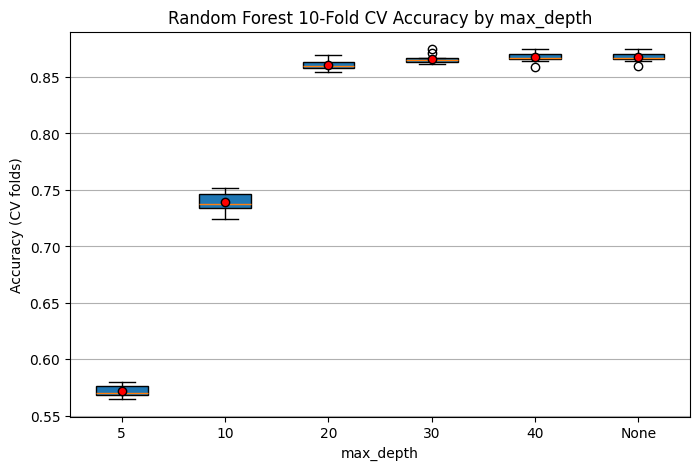
\includegraphics[width=0.8\textwidth]{figures/rf_accuracy_kfold.png}
\caption{Accuracy of Random Forest classifier with K-Fold Cross-validation. Each box and whisker plots shows the spread of the accuracy against the test data across the 10 folds. The red line shows the mean accuracy across the 10 folds.}
\label{fig:rf_accuracy_kfold}
\end{figure}

The distribution of the accuracy shows a low variance across all maximum depths, which suggests that the Random Forest classifier is not overfitting the data. The maximum depth of None (unlimited) acheived the highest mean accuracy, while still maintaining a low variance, therefore we will use this model as the standard model for the Random Forest classifier. 
\\
Note that the mean of the accuracies for maximum depths larger than 20 are very similar. Additionally, the mean accuracy for 40 is within the IQR of the maximum depth of None. It is fair to assume the true mean across the maximum depths larger than 20 are insignficantly different, and so the choice of maximum depth greater than 20 is arbitrary, in terms of accuracy. Despite the fact that the computational time is significantly increased as the maximum depth increases, we will use the maximum depth of None, because the time taken is within reason, and the accuracy, for this dataset, is the highest.

\vspace{20pt}

\textbf{6.3 ROC curve}
\\

% Insert figure of RF ROC curve here
\begin{figure}[H]
\centering
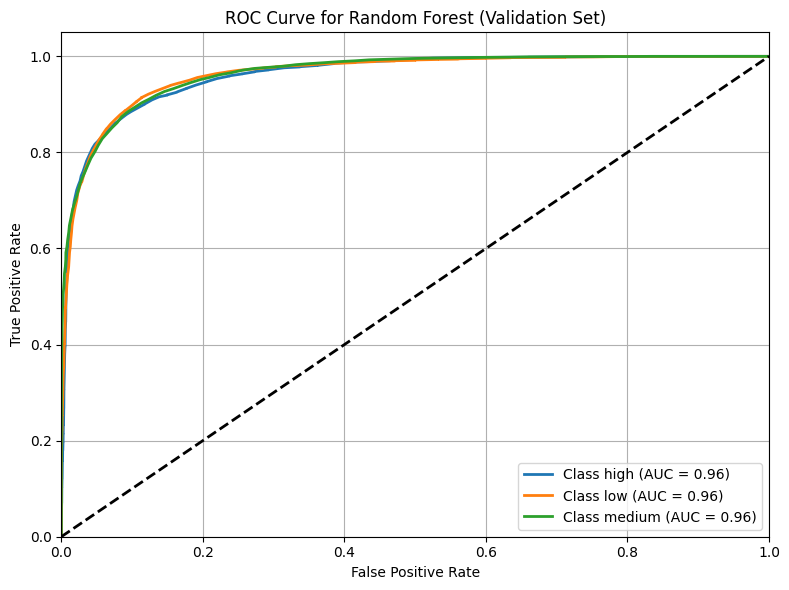
\includegraphics[width=0.8\textwidth]{figures/rf_roc_curve.png}
\caption{ROC curve for Random Forest classifier with 100 trees and maximum depth of None.}
\label{fig:rf_roc_curve}
\end{figure}

The ROC curve for the Random Forest classifier with 100 trees and unlimited depth is shown in Figure \ref{fig:rf_roc_curve}. The area under the curve (AUC) is approximately 0.96 for all height categories, indicating strong discriminative performance with a high true positive rate and a low false positive rate across classes. Notably, the Random Forest achieves a higher AUC than the K-NN classifier with (k=1), suggesting superior classification performance on this dataset. 
\\
This improvement is consistent with the strengths of ensemble methods like Random Forest, which aggregate the predictions of multiple decision trees to reduce variance and improve generalization. Additionally, Random Forests are less prone to overfitting compared to single decision trees, particularly when a sufficient number of trees are used.

\vspace{20pt}

\textbf{6.4 Confusion matrix}
\\
% Insert figure of RF confusion matrix here
\begin{figure}[H]
\centering
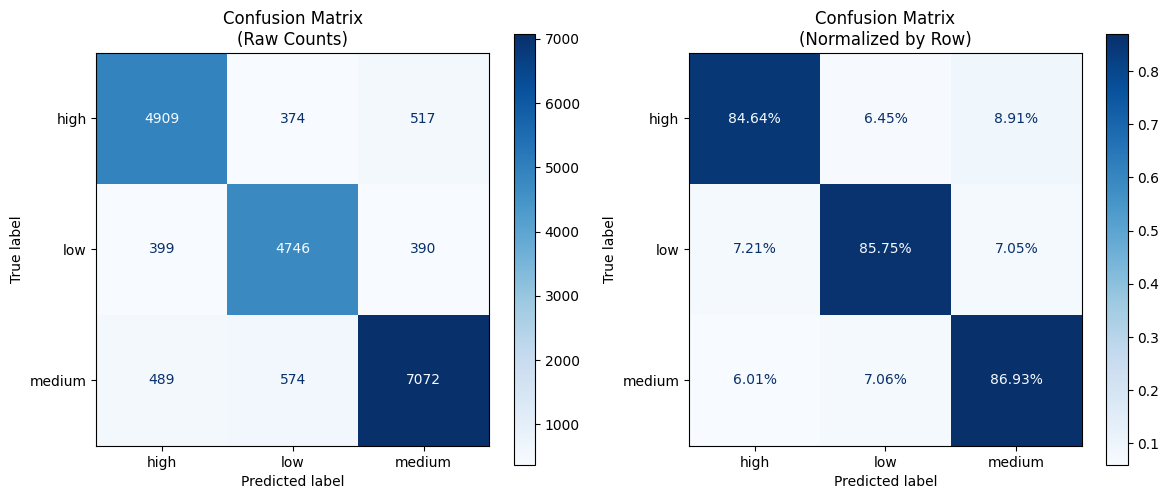
\includegraphics[width=1\textwidth]{figures/rf_confusion_matrix.png}
\caption{Confusion matrix for Random Forest classifier with 100 trees and maximum depth of None. (Left) Confusion matrix against the raw validation set. (Right) Confusion matrix normalized by row.}
\label{fig:rf_confusion_matrix}
\end{figure}

Similar to the K-NN classifier, the diagonal elements are the largest, which indicates that the Random Forest classifier with 100 trees and unlimited depth is able to correctly classify the majority of the data points. 
\\
The diagonal elements for the Random Forest classifier are slightly lower than the K-NN classifier, which indicates that the chosen Random Forest classifier is only slightly less accurate than the K-NN classifier.

\vspace{20pt}

\textbf{6.5 Precision, Recall, and F1 score}
\\

\begin{table}[h!]
\centering
\begin{tabular}{lcccc}
\hline
\textbf{Class} & \textbf{Precision} & \textbf{Recall} & \textbf{F1-score} \\
\hline
high   & 0.85 & 0.85 & 0.85 & \\
low    & 0.83 & 0.86 & 0.85 & \\
medium & 0.89 & 0.87 & 0.88 & \\
\hline
\end{tabular}
\caption{Precision, recall, and F1-score for each class on the validation set.}
\label{tab:rf_classification_report}
\end{table}

The precision, recall, and F1 score are very similar to that of the K-NN classifier and are all high for all three classes, which indicates that the Random Forest classifier with 100 trees and unlimited depth is able to correctly classify the majority of the data points in each category. Additionally, the scores are relatively balanced across all classes, which suggests that the Random Forest classifier with 100 trees and unlimited depth is not biased towards any particular class.

\vspace{20pt}

\textbf{7. Deep Neural Networks}
\\
The Deep Neural Network (DNN) is a powerful machine learning algorithm that can be used for both classification and regression tasks. The DNN algorithm works by using multiple layers of neurons to learn complex decision boundaries. For this section, we will explore two-hidden layer DNNs, which are a type of feedforward neural network. The model is trained using the Cross Entropy loss function, with a L2 regularization term to prevent overfitting. The model is trained using the Adam optimizer, which is a popular optimization algorithm for training neural networks. The model is trained on the scaled training data, and then tested on the testing data.

\vspace{20pt}

\textbf{7.1 Training}
\\
Initial assessment of the DNN were performed using a 128 nodes in each hidden layers. It was found that the DNN can acheive a accuracy on-par with the previous models when trained using a batch size of 16, learning rate of 0.001, and 100 epochs. However, it is unclear if the model is overfitting, and so we will use 5-fold cross-validation to investigate the effect of the different hidden layer sizes on the accuracy of the DNN.

\textbf{7.1.1 Effect of hidden layer sizes}


% Insert Figure of DNN training here with 5-fold cross-validation
\begin{figure}[H]
\centering
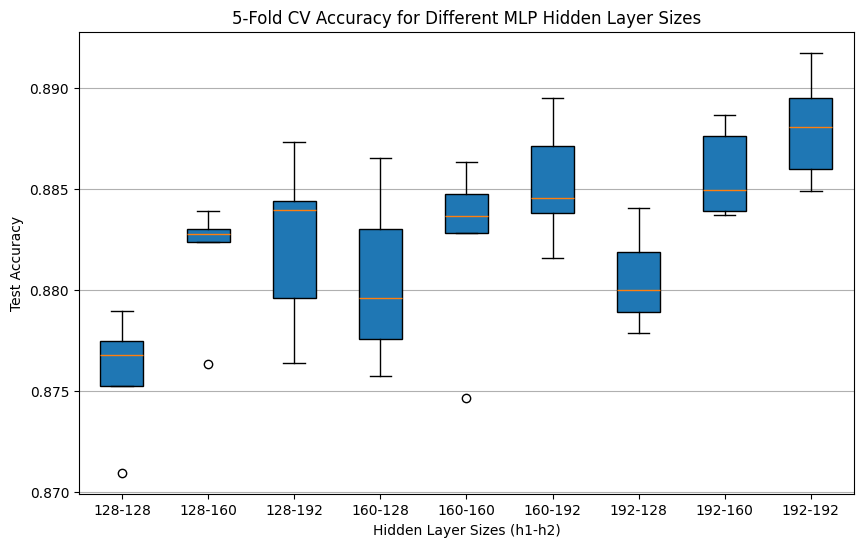
\includegraphics[width=0.8\textwidth]{figures/dnn_crossval.png}
\caption{Different hidden layer sizes (h1-h2) with 5-fold cross-validation. Each box and whisker plots shows the spread of the accuracy against the test data across the 5 folds. The red line shows the mean accuracy across the 5 folds.}
\label{fig:dnn_training}
\end{figure}

There appears to be a trend for increasing the size of the hiddens layers to increase the accuracy of the DNN. Notably, the biggest increase in accuracies occurs when the second hidden layer is increased, for the same size of the first hidden layer. This suggests that the second hidden layer is more important than the first hidden layer, and that increasing the size of the second hidden layer will increase the accuracy of the DNN.
\\
The DNN with 192-192 hidden layers has the higest mean accuracy, and has a low variance, that is comparable to the other models. This suggest that the DNN with 192-192 hidden layers is a good choice for this dataset, and that the DNN is not overfitting the data, or at least not overfitting the data more than the other models.


\end{document}
